\chapter{Functionele organisatie van een zoogdier}\label{ch:b1:mammal-organization}

Open een konijn op de snijtafel en de eerste indruk is die van orde. Een
spierplaat, het \omterm{def:b1:mammal-organization:bodyplan}{middenrif}, verdeelt de romp in een borstholte met het hart en
twee longen en een buikholte met al de rest: een lever ter grootte van een
vuist, een maag, vier meter darm die eindigt in een blindedarm zo groot als de
maag, en twee nieren tegen de achterwand. Elk \omterm{def:b1:mammal-organization:organ}{orgaan} heeft een plaats, een
bloedvoorziening en een taak; geen ervan werkt alleen. Dit hoofdstuk beschrijft
hoe het zoogdier als functionerend geheel is gebouwd: zijn \omterm{def:b1:mammal-organization:bodyplan}{bouwplan}, de
stelsels waarin zijn \omterm{def:b1:mammal-organization:organ}{organen} zijn gegroepeerd, de vloeistofcompartimenten
waarin zijn cellen leven, de \omterm{prop:b1:organism-environment:surfaces}{uitwisselingsoppervlakken} waarmee het de
buitenwereld ontmoet, en de \omterm{prop:b1:mammal-organization:heatbudget}{warmtebalans} die het op \qty{39}{\celsius} houdt in
een januariweide.

\section{Het bouwplan van een zoogdier}

\begin{definition}[Bouwplan]\label{def:b1:mammal-organization:bodyplan}
Het \emph{bouwplan}\index{bouwplan} van een dier is de rangschikking van zijn
assen, holten en \omterm{def:b1:mammal-organization:organ}{organen} die alle leden van zijn groep gemeen hebben. Het
bouwplan van de zoogdieren is dat van een gewervelde: bilaterale symmetrie met
een kopeinde dat de hersenen en de belangrijkste zintuigen draagt
(\emph{cefalisatie}\index{cefalisatie}), een rugas van wervels rond het
ruggenmerg, vier ledematen, en een buikzijdige lichaamsholte --- het
\emph{coeloom}\index{coeloom} --- met daarin de ingewanden. Specifiek voor
zoogdieren is: het coeloom is door het gespierde
\emph{middenrif}\index{middenrif} verdeeld in een borstholte (hart, longen) en
een buikholte (verteringsorganen, nieren, geslachtsklieren); het lichaam is met
haren bedekt; de jongen worden met melk gevoed; de temperatuur wordt geregeld.
\end{definition}

\begin{omfigure}
\begin{tikzpicture}
  \node[anchor=south west, inner sep=0] (img) at (0,0)
    {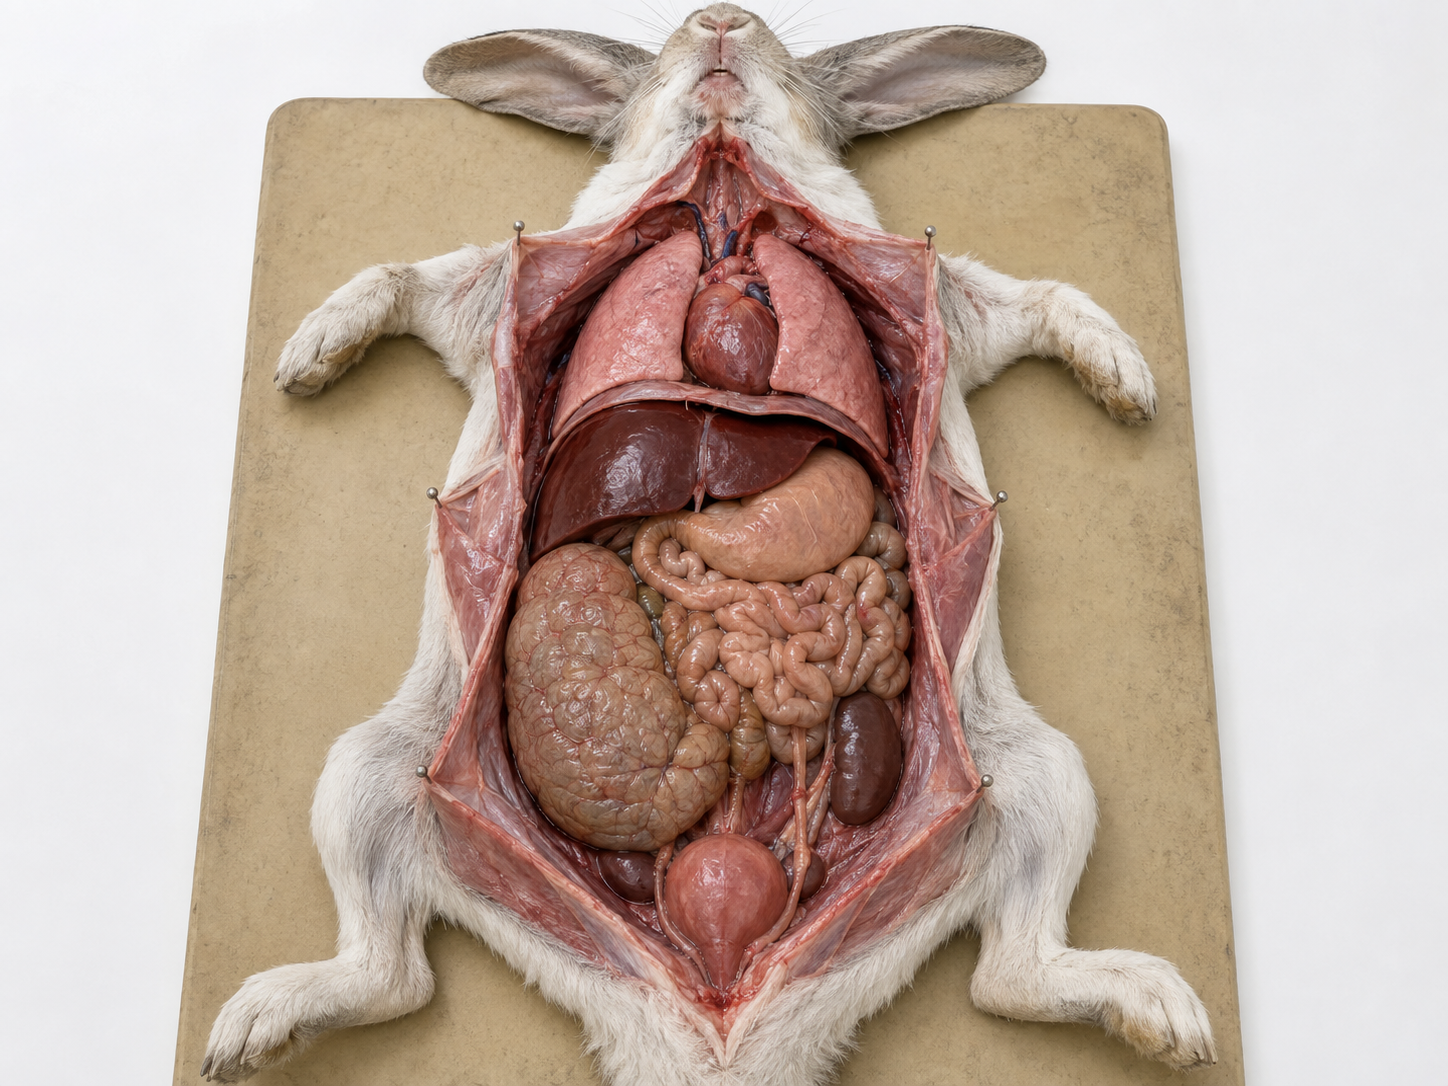
\includegraphics[width=0.6\linewidth]{images/book3/ai/fig-rabbit-dissection.png}};
  \begin{scope}[x={(img.south east)}, y={(img.north west)},
      every node/.style={font=\small}]
    \draw[omDef, thick] (0.44,0.72) -- (-0.02,0.90) node[left] {longen};
    \draw[omDef, thick] (0.50,0.68) -- (1.02,0.88) node[right] {hart};
    \draw[omDef, thick] (0.53,0.61) -- (1.02,0.70) node[right] {middenrif};
    \draw[omDef, thick] (0.44,0.55) -- (-0.02,0.62) node[left] {lever};
    \draw[omDef, thick] (0.56,0.52) -- (1.02,0.54) node[right] {maag};
    \draw[omDef, thick] (0.52,0.42) -- (1.02,0.40) node[right] {dunne darm};
    \draw[omDef, thick] (0.42,0.36) -- (-0.02,0.36) node[left] {blindedarm};
    \draw[omDef, thick] (0.60,0.30) -- (1.02,0.24) node[right] {nier};
    \draw[omDef, thick] (0.51,0.17) -- (-0.02,0.10) node[left] {blaas};
  \end{scope}
\end{tikzpicture}

{\small Een konijn geopend vanaf de buikzijde. Het \omterm{def:b1:mammal-organization:bodyplan}{middenrif} scheidt de
borstholte (longen, hart) van de buikholte (lever, maag, darm, blindedarm,
nieren, blaas). Elk \omterm{def:b1:mammal-organization:organ}{orgaan} ligt op een vaste plaats, omhuld door een vlies en
bediend door zijn eigen bloedvaten.}
\end{omfigure}

\begin{definition}[Orgaan, orgaanstelsel]\label{def:b1:mammal-organization:organ}
Een \emph{orgaan}\index{orgaan} is een structuur van verschillende weefsels
(\cref{ch:b1:body-plans-tissues}) die zo zijn geschikt dat zij een bepaalde
functie vervullen: het hart pompt, de long wisselt gassen uit, de nier filtert.
Een \emph{orgaanstelsel}\index{orgaanstelsel} is een verzameling organen die
samenwerken in één brede functie: het spijsverteringsstelsel loopt van mond tot
anus met de lever en de alvleesklier eraan verbonden; het bloedvatenstelsel is
het hart met de bloedvaten; het uitscheidingsstelsel de nieren en de urinewegen.
\end{definition}

\section{Orgaanstelsels en de functies die zij vervullen}

\begin{proposition}[Drie groepen functies]\label{prop:b1:mammal-organization:functions}
De \omterm{def:b1:mammal-organization:organ}{orgaanstelsels} van een zoogdier vervullen drie groepen functies:
\begin{itemize}
  \item \emph{voeding}\index{voedingsfunctie}: materie en energie opnemen
        en verdelen en afvalstoffen kwijtraken --- het spijsverterings-,
        ademhalings-, bloedvaten- en uitscheidingsstelsel;
  \item \emph{relatie}\index{relatiefunctie}: de omgeving waarnemen en
        erop inwerken --- de zintuigen, het zenuwstelsel, de
        hormoonklieren, het skelet en de spieren;
  \item \emph{voortplanting}\index{voortplantingsfunctie}: nakomelingen
        voortbrengen --- de geslachtsklieren, de geslachtswegen en, bij
        zoogdieren, de melkklieren.
\end{itemize}
Geen enkel stelsel werkt alleen: elk \omterm{def:b1:mammal-organization:organ}{orgaan} is voor zijn aanvoer afhankelijk
van het bloed, voor zijn afstemming van het zenuwstelsel en de hormoonklieren,
en voor zijn bescherming van het skelet en de huid.
\end{proposition}

\begin{omfigure}
\begin{tikzpicture}[font=\footnotesize, >=Stealth, line cap=round,
  sys/.style={draw, thick, rounded corners=3pt, minimum height=7mm, minimum width=24mm, align=center, fill=white},
  lab/.style={font=\scriptsize, above},
  grp/.style={font=\small\bfseries, anchor=west}]
  \node[grp, omProp] at (0,4.6) {Voeding};
  \node[sys, fill=omProp!12] (dig) at (1.3,3.8) {spijsvertering};
  \node[sys, fill=omProp!12] (res) at (1.3,2.9) {ademhaling};
  \node[sys, fill=omProp!12] (exc) at (1.3,2.0) {uitscheiding};
  \node[grp, omExo] at (0,1.1) {Voortplanting};
  \node[sys, fill=omExo!12] (gen) at (1.3,0.3) {geslachtsorganen};
  \node[sys, fill=omThm!12, minimum height=30mm] (cir) at (5.9,2.6) {bloedvaten\\ (bloed, lymfe)};
  \node[grp, omDef] at (8.6,4.6) {Relatie};
  \node[sys, fill=omDef!12, minimum width=30mm] (ner) at (10.3,3.8) {zenuwen, zintuigen};
  \node[sys, fill=omDef!12, minimum width=30mm] (end) at (10.3,2.9) {hormoonklieren};
  \node[sys, fill=omDef!12, minimum width=30mm] (mus) at (10.3,2.0) {skelet, spieren};
  \node[sys, fill=omDef!12, minimum width=30mm] (ski) at (10.3,1.1) {huid};
  \draw[<->, thick] (dig.east) -- (cir.west |- dig.east) node[lab, midway] {voedingsstoffen};
  \draw[<->, thick] (res.east) -- (cir.west |- res.east) node[lab, midway] {$\mathrm{O_2}$, $\mathrm{CO_2}$};
  \draw[<->, thick] (exc.east) -- (cir.west |- exc.east) node[lab, midway] {afvalstoffen};
  \draw[<->, thick] (gen.east) -- ++(1.6,0) |- (cir.south west);
  \draw[<->, thick] (cir.east |- ner.west) -- (ner.west);
  \draw[<->, thick] (cir.east |- end.west) -- (end.west) node[lab, midway] {hormonen};
  \draw[<->, thick] (cir.east |- mus.west) -- (mus.west);
  \draw[<->, thick] (cir.south east) -| ++(0.5,0) |- (ski.west);
\end{tikzpicture}

{\small De \omterm{def:b1:mammal-organization:organ}{orgaanstelsels} van een zoogdier, gegroepeerd naar functie. De
bloedsomloop is het knooppunt: elk stelsel wisselt uit met het bloed, en het
bloed brengt wat het ene stelsel opneemt naar alle andere.}
\end{omfigure}

\begin{example}[Een hap gras]\label{ex:b1:mammal-organization:mouthful}
Het gras van het konijn wordt door de snijtanden afgeknipt en door de kiezen
vermalen (skelet en spieren), geproefd en geroken (zintuigen), doorgeslikt en
verteerd in de maag en de dunne darm; de suikers en aminozuren gaan door de
darmwand het bloed in en bereiken de lever, die ze onder hormonale sturing
opslaat of afgeeft (hormoonklieren); de cellulose wordt door bacteriën in de
blindedarm vergist; de zuurstof om de suikers te verbranden komt via de longen
binnen, de koolstofdioxide vertrekt langs dezelfde weg, het ureum uit de
aminozuren verlaat het lichaam via de nieren, en de warmte van het hele proces
via de huid. Zeven stelsels voor één hap.
\end{example}

\section{De compartimenten van het lichaam}

\begin{definition}[Vloeistofcompartimenten]\label{def:b1:mammal-organization:compartments}
Water maakt ongeveer \qty{60}{\%} van de massa van een zoogdier uit. Twee derde
daarvan is \emph{intracellulaire vloeistof}\index{intracellulaire vloeistof},
binnen de cellen; een derde is
\emph{extracellulaire vloeistof}\index{extracellulaire vloeistof}, het \omterm{def:b1:organism-environment:milieu}{intern
milieu} van \cref{ch:b1:organism-environment}, dat zelf uiteenvalt in de
\emph{interstitiële vloeistof}\index{interstitiële vloeistof} die de cellen
omspoelt (drie kwart ervan) en het \emph{bloedplasma}\index{plasma} in de bloedvaten
(een kwart). \emph{Lymfe}\index{lymfe} is interstitiële vloeistof die door de
lymfevaten wordt opgehaald en aan het bloed teruggegeven. De twee
extracellulaire vloeistoffen hebben vrijwel dezelfde samenstelling --- plasma
verschilt door zijn eiwitten, die de haarvatwand niet passeren --- en beide
verschillen scherp van de intracellulaire vloeistof.
\end{definition}

\begin{omfigure}
\begin{tikzpicture}[font=\small, line cap=round]
  \draw[thick, fill=gray!8, rounded corners=6pt] (0,0) rectangle (11.6,4.6);
  \node[anchor=north west, font=\small\bfseries] at (0.15,4.55) {totaal lichaamswater: \qty{42}{L} (\qty{60}{\%} van \qty{70}{kg})};
  \draw[thick, fill=omDef!14, rounded corners=5pt] (0.3,0.3) rectangle (6.4,3.8);
  \node[anchor=north west, align=left] at (0.4,3.7) {\textbf{intracellulaire vloeistof}: \qty{28}{L}\\ veel $\mathrm{K^+}$ (\qty{140}{mmol/L}),\\ fosfaat, eiwitten;\\ weinig $\mathrm{Na^+}$ (\qty{10}{mmol/L})};
  \draw[thick, fill=omProp!14, rounded corners=5pt] (6.7,0.3) rectangle (11.3,3.8);
  \node[anchor=north west, align=left] at (6.8,3.7) {\textbf{extracellulaire vloeistof}: \qty{14}{L}\\ veel $\mathrm{Na^+}$ (\qty{140}{mmol/L}),\\ $\mathrm{Cl^-}$, $\mathrm{HCO_3^-}$};
  \draw[thick, fill=omProp!30, rounded corners=4pt] (6.9,0.45) rectangle (9.2,1.55);
  \node[align=center, font=\footnotesize] at (8.05,1.0) {interstitieel\\ \qty{11}{L}};
  \draw[thick, fill=omThm!30, rounded corners=4pt] (9.4,0.45) rectangle (11.1,1.55);
  \node[align=center, font=\footnotesize] at (10.25,1.0) {plasma\\ \qty{3}{L}};
\end{tikzpicture}

{\small De vloeistofcompartimenten van een mens van \qty{70}{kg}. Twee derde
van het water zit binnen de cellen; het extracellulaire derde, verdeeld over de
\omterm{def:b1:mammal-organization:compartments}{interstitiële vloeistof} en het \omterm{def:b1:mammal-organization:compartments}{plasma}, is het \omterm{def:b1:organism-environment:milieu}{intern milieu}. Buiten overheerst
natrium, binnen kalium --- een verschil dat elke cel energie kost om in stand
te houden (\cref{ch:b1:membranes-transport}).}
\end{omfigure}

\begin{method}[Een compartiment meten door verdunning]\label{met:b1:mammal-organization:dilution}
\begin{enumerate}
  \item Kies een merkstof die zich over het compartiment verdeelt en
        nergens anders komt: een kleurstof die aan plasma-eiwitten bindt
        (evansblauw) voor het \omterm{def:b1:mammal-organization:compartments}{plasma}; inuline, een suiker die de bloedvaten
        verlaat maar niet in de cellen komt, voor de \omterm{def:b1:mammal-organization:compartments}{extracellulaire
        vloeistof}; zwaar water voor het totale lichaamswater.
  \item Spuit een bekende hoeveelheid $m$ in en wacht tot de menging
        voltooid is (minuten voor \omterm{def:b1:mammal-organization:compartments}{plasma}, uren voor het totale water).
  \item Meet de concentratie $c$ in een plasmamonster en corrigeer voor
        eventueel verlies (urine, stofwisseling) tijdens het wachten.
  \item Het volume is $V = m/c$. Het intracellulaire volume is het totale
        water min het extracellulaire; het interstitiële volume is het
        extracellulaire min het \omterm{def:b1:mammal-organization:compartments}{plasma}. Het bloedvolume is het
        plasmavolume gedeeld door de plasmafractie van het bloed
        ($1 - $ hematocriet).
\end{enumerate}
\end{method}

\begin{example}[Een plasmavolume]\label{ex:b1:mammal-organization:evansblue}
\qty{50}{mg} evansblauw, ingespoten bij een man van \qty{70}{kg}, geeft tien
minuten later een plasmaconcentratie van \qty{16.7}{mg/L}:
$V = 50/16.7 = \qty{3.0}{L}$ \omterm{def:b1:mammal-organization:compartments}{plasma}. Met een hematocriet van \qty{45}{\%} is
het bloedvolume $3.0/0.55 = \qty{5.5}{L}$ --- \qty{8}{\%} van de
lichaamsmassa, een verhouding die van muis tot walvis geldt.
\end{example}

\section{Uitwisselingsoppervlakken en de bloedsomloop}

\begin{proposition}[Elk uitwisselingsoppervlak is aan het bloed gekoppeld]\label{prop:b1:mammal-organization:surfaces}
Een zoogdier wisselt met de buitenwereld uit via vier oppervlakken, elk in het
lichaam opgevouwen en elk doorstroomd door een dicht haarvatennet: het
darmslijmvlies (\qty{30}{m^2} bij een mens) voor voedingsstoffen en water, het
longblaasjesoppervlak van de longen (\qty{100}{m^2}) voor zuurstof en
koolstofdioxide, het filteroppervlak van de nieren (een miljoen glomeruli, die
\qty{180}{L} \omterm{def:b1:mammal-organization:compartments}{plasma} per dag filtreren) voor afvalstoffen en de regeling van het
\omterm{def:b1:organism-environment:milieu}{intern milieu}, en de huid (\qty{2}{m^2}) voor warmte en een beetje water. De
bloedsomloop verbindt ze: bloed dat het ene oppervlak verlaat bereikt het
volgende binnen een minuut, zodat wat via de darm binnenkomt wordt geoxideerd
met zuurstof uit de long en zijn afval via de nier vertrekt.
\end{proposition}

\begin{omfigure}
\begin{tikzpicture}[font=\small, >=Stealth, line cap=round,
  org/.style={draw, thick, rounded corners=4pt, minimum height=8mm, minimum width=22mm, align=center, fill=white}]
  \node[org, fill=omDef!12] (lung) at (0,3.2) {longen\\ \qty{100}{m^2}};
  \node[org, fill=omThm!15, minimum width=26mm, minimum height=12mm] (heart) at (0,0) {hart\\ rechts $\mid$ links};
  \node[org, fill=omProp!12] (gut) at (5.2,1.6) {darm\\ \qty{30}{m^2}};
  \node[org, fill=omProp!12] (liver) at (5.2,0.0) {lever};
  \node[org, fill=omProp!12] (kid) at (5.2,-1.6) {nieren\\ \qty{180}{L/d}};
  \node[org, fill=omExo!12] (mus) at (5.2,3.2) {spieren, huid,\\ hersenen, overige};
  % pulmonary loop
  \draw[->, very thick, omDef] (heart.north west) ++(-0.2,0) |- (lung.west) node[pos=0.25, left, font=\footnotesize, align=right] {kleine\\ bloedsomloop};
  \draw[->, very thick, omThm] (lung.east) -| ($(heart.north east)+(0.2,0)$);
  % systemic loop: left heart -> organs (parallel) -> right heart
  \draw[very thick, omThm] (heart.east) -- ++(1.2,0) coordinate (a);
  \draw[->, very thick, omThm] (a) |- (mus.west);
  \draw[->, very thick, omThm] (a) |- (gut.west);
  \draw[->, very thick, omThm] (a) |- (kid.west);
  \draw[->, very thick, omThm] (a) -- (liver.west);
  \draw[->, very thick, omDef] (gut.south) -- (liver.north) node[midway, right, font=\footnotesize] {poortader};
  \coordinate (b) at (8.0,0.8);
  \draw[very thick, omDef] (mus.east) -| (b);
  \draw[very thick, omDef] (liver.east) -| (b);
  \draw[very thick, omDef] (kid.east) -| (b);
  \draw[->, very thick, omDef] (b) |- ++(0,-3.2) -| (heart.south) node[pos=0.25, below, font=\footnotesize] {grote bloedsomloop: aders};
\end{tikzpicture}

{\small De dubbele bloedsomloop van een zoogdier. Het rechterhart stuurt
zuurstofarm bloed (blauw) door de longen; het linkerhart stuurt zuurstofrijk
bloed (rood) door de \omterm{def:b1:mammal-organization:organ}{organen}, die parallel geschakeld zijn, zodat elk vers
slagaderlijk bloed ontvangt. Bloed uit de darm passeert de lever voordat het
naar het hart terugkeert.}
\end{omfigure}

\begin{omfigure}
\begin{tikzpicture}
\begin{axis}[
  xbar, bar width=8pt,
  width=0.82\linewidth, height=6.2cm,
  axis x line=bottom, axis y line=left,
  xmin=0, xmax=1.8, xlabel={bloedstroom in rust (\unit{L/min})},
  xlabel style={font=\small, at={(axis description cs:0.5,-0.13)}, anchor=north},
  symbolic y coords={hartspier, huid, hersenen, skeletspier, nieren, lever en darm},
  ytick=data, tick label style={font=\small},
  enlarge y limits=0.12, xtick={0,0.5,1.0,1.5},
  nodes near coords, nodes near coords style={font=\scriptsize, anchor=west},
]
\addplot[fill=omThm!45, draw=omThm] coordinates
  {(0.25,hartspier) (0.4,huid) (0.75,hersenen) (1.0,skeletspier) (1.1,nieren) (1.35,lever en darm)};
\end{axis}
\end{tikzpicture}

{\small Hoe een hartminuutvolume van \qty{5}{L/min} bij een mens in rust over
de \omterm{def:b1:mammal-organization:organ}{organen} wordt verdeeld. De nieren, \qty{0.5}{\%} van de lichaamsmassa,
nemen een vijfde van het bloed --- de prijs van het zestig keer per dag
filtreren van het hele \omterm{def:b1:mammal-organization:compartments}{plasma}. Tijdens inspanning stijgt het aandeel van de
spieren tienvoudig en daalt dat van de darm.}
\end{omfigure}

\begin{example}[De omlooptijd]\label{ex:b1:mammal-organization:circtime}
Met \qty{5.5}{L} bloed en een hartminuutvolume van \qty{5}{L/min} legt een
druppel bloed de dubbele kringloop in rust in ongeveer één minuut af, en bij
zware inspanning in een kwart daarvan, wanneer het minuutvolume
\qty{20}{L/min} bereikt. Het hartminuutvolume schaalt als $M^{3/4}$
(\cref{thm:b1:organism-environment:kleiber}): dat van een konijn van
\qty{2}{kg} is ongeveer \qty{0.35}{L/min} voor \qty{160}{mL} bloed --- op een
factor twee na dezelfde omlooptijd, bij een hartslagfrequentie van
\qty{200}{} slagen per minuut.
\end{example}

\section{Endothermie en de warmtebalans}

\begin{proposition}[De warmtebalans]\label{prop:b1:mammal-organization:heatbudget}
\index{warmtebalans}
Een zoogdier op stabiele temperatuur voldoet aan
\[
M - W = R + C + K + E ,
\]
waarin $M$ de warmteproductie door de stofwisseling is, $W$ de mechanische
arbeid op de buitenwereld, en het rechterlid de verliezen door straling $R$,
convectie naar de lucht $C$, geleiding naar de bodem $K$ en verdamping $E$
(uit de longen, en door zweten of hijgen). De eerste drie verliezen zijn
evenredig met $T_b - T_a$ en worden bepaald door de isolatie van de vacht en de
doorbloeding van de huid; verdamping is de enige weg die nog werkt wanneer de
lucht warmer is dan het lichaam. Wanneer de vergelijking niet is voldaan,
verschuift de lichaamstemperatuur met een snelheid die door de onbalans en door
de warmtecapaciteit van het lichaam wordt bepaald (ongeveer
\qty{3.5}{kJ.kg^{-1}.K^{-1}}).
\end{proposition}
\begin{proof}
Behoud van energie voor het lichaam over een periode waarin zijn temperatuur
niet verandert: de vrijgekomen chemische energie ($M$) vertrekt als arbeid of
als warmte via de vier fysische kanalen. De evenredigheid van $R$, $C$ en $K$
met het temperatuurverschil is de afkoelingswet van Newton
(\cref{ch:b1:organism-environment}); dat $E$ onafhankelijk is van dat verschil
volgt eruit dat verdamping wordt aangedreven door de vochtgradiënt en niet door
de temperatuurgradiënt.
\end{proof}

\begin{omfigure}
\begin{tikzpicture}[font=\small, >=Stealth, line cap=round]
  \draw[very thick, fill=omThm!8, rounded corners=16pt] (0,0) rectangle (5.0,3.0);
  \node[align=center] at (2.5,1.5) {lichaamskern \qty{39}{\celsius}\\ warmteproductie $M$\\ (basaal, rillen, activiteit)};
  \draw[->, very thick, omThm] (5.0,2.5) -- (6.6,2.5) node[right, align=left] {$R$: straling naar\\ wanden en hemel};
  \draw[->, very thick, omThm] (5.0,1.8) -- (6.6,1.8) node[right, align=left] {$C$: convectie naar de lucht};
  \draw[->, very thick, omThm] (5.0,1.1) -- (6.6,1.1) node[right, align=left] {$K$: geleiding naar de bodem};
  \draw[->, very thick, omDef] (5.0,0.4) -- (6.6,0.4) node[right, align=left] {$E$: verdamping\\ (adem, zweet)};
  \draw[->, very thick, omExo] (-1.6,1.5) -- (0,1.5) node[pos=0, left, align=right] {voedselenergie\\ (en opgeslagen vet)};
  \draw[->, very thick, gray] (2.5,0) -- (2.5,-0.9) node[below, align=center] {$W$: arbeid op de buitenwereld};
  \node[font=\footnotesize, align=center, anchor=south] at (2.5,3.1) {vacht en huiddoorbloeding\\ bepalen $R$, $C$, $K$;\\ zij zijn $\propto (T_b - T_a)$};
\end{tikzpicture}

{\small De \omterm{prop:b1:mammal-organization:heatbudget}{warmtebalans} van een \omterm{prop:b1:organism-environment:thermo}{endotherm}. De productie moet gelijk zijn aan de
som van de vier verliezen plus de uitwendige arbeid; het dier stelt de productie
(rillen, activiteit), de isolatie (vacht, houding, huiddoorbloeding) en de
verdamping bij om de balans te bewaren.}
\end{omfigure}

\begin{proposition}[De middelen van de warmteregeling]\label{prop:b1:mammal-organization:thermoreg}
Tegen kou beperkt een zoogdier het verlies --- het zet zijn vacht op, vernauwt
de bloedvaten van de huid en de uitsteeksels, rolt zich op, kruipt bij elkaar ---
en verhoogt het de productie: rillen (ritmische samentrekking van de spieren)
en, bij kleine en jonge zoogdieren, \emph{niet-rillende
warmteproductie}\index{niet-rillende warmteproductie} in \emph{bruin
vetweefsel}\index{bruin vetweefsel}, waarvan de mitochondriën de energie van
vet rechtstreeks als warmte vrijgeven. Tegen warmte verwijdt het de huidvaten
(de oren van een konijn kunnen een derde van zijn warmte lozen) en verdampt het
water door te zweten (paard, mens) of te hijgen (hond, konijn). Dit alles wordt
aangestuurd vanuit de hypothalamus, die de \omterm{def:b1:organism-environment:homeostasis}{streefwaarde} vasthoudt en de
temperatuur van het bloed en van de huid afleest.
\end{proposition}
\begin{proof}[Bewijsmateriaal]
Wanneer de hypothalamus van een hond met een ingebrachte sonde wordt verwarmd,
gaat hij hijgen en zijn huidvaten verwijden in een koude kamer; koelt men de
sonde af, dan gaat hij rillen in een warme kamer. Het zuurstofverbruik van een
rat die bij \qty{5}{\celsius} wordt gezet verdrievoudigt binnen een uur, de
helft van de toename door rillen (geregistreerd als elektrische spieractiviteit)
en de helft door bruin vet, waarvan de temperatuur, met een thermokoppel
gemeten, die van de omringende weefsels overtreft. Infraroodbeelden van een
konijn bij \qty{30}{\celsius} tonen zijn oren op bijna lichaamstemperatuur, bij
\qty{5}{\celsius} op bijna luchttemperatuur.
\end{proof}

\begin{example}[De oren van het konijn]\label{ex:b1:mammal-organization:ears}
Twee oren van elk ongeveer \qty{50}{cm^2}, dun, bijna kaal en rijk doorbloed:
met hun bloedvaten open bij \qty{30}{\celsius} in lucht van \qty{20}{\celsius} en
met een coëfficiënt voor kale huid van \qty{10}{W.m^{-2}.K^{-1}} verliezen zij
$10\times 0.01\times 10 =
\qty{1}{W}$, een zesde van de productie van een rustend konijn. Bij
\qty{5}{\celsius} sluiten de bloedvaten, koelen de oren af tot bijna
luchttemperatuur, en daalt het verlies erdoor tot onder \qty{0.2}{W}.
\end{example}

\begin{remark}[Afstemming]\label{rem:b1:mammal-organization:coordination}
Elke bijstelling hierboven --- een vat dat vernauwt, een spier die rilt, een
klier die afscheidt --- is een opdracht die door een zenuw of een hormoon wordt
overgebracht. Het zenuwstelsel werkt in milliseconden langs vaste banen; het
hormoonstelsel werkt in minuten tot uren via het bloed en bereikt elke cel die
de juiste receptor draagt. Hun mechanismen zijn het onderwerp van het deel van
jaar 2; dit jaar neemt ze als gegeven aan en bestudeert wat zij afstemmen.
\end{remark}

\section{Opgaven}

\begin{exercise}[$\star$]\label{exo:b1:mammal-organization:1}
Noem de kenmerken van het \omterm{def:b1:mammal-organization:bodyplan}{bouwplan} van de zoogdieren die zij met alle
gewervelden delen, en die welke voor zoogdieren specifiek zijn.
\end{exercise}

\begin{exercise}[$\star$]\label{exo:b1:mammal-organization:2}
Wijs elk \omterm{def:b1:mammal-organization:organ}{orgaanstelsel} toe aan een van de drie groepen functies, en noem van
elk stelsel één \omterm{def:b1:mammal-organization:organ}{orgaan}.
\end{exercise}

\begin{exercise}[$\star$]\label{exo:b1:mammal-organization:3}
Een vrouw van \qty{60}{kg}: schat haar totale lichaamswater, haar
intracellulaire en extracellulaire volume, haar interstitiële volume en haar
plasmavolume.
\end{exercise}

\begin{exercise}[$\star$]\label{exo:b1:mammal-organization:4}
Welk deel van het hartminuutvolume gaat volgens de figuur van de bloedstroom
naar de nieren, en hoe vaak per dag wordt het hele bloedvolume
(\qty{5.5}{L}) erdoorheen gepompt?
\end{exercise}

\begin{exercise}[$\star\star$]\label{exo:b1:mammal-organization:5}
Bij een man van \qty{70}{kg} wordt \qty{2.0}{g} inuline ingespoten; na menging,
en nadat \qty{0.3}{g} met de urine verloren is gegaan, bedraagt de
plasmaconcentratie \qty{0.12}{g/L}. Bereken het extracellulaire volume, en, met
een totaal water van \qty{42}{L}, het intracellulaire volume.
\end{exercise}

\begin{exercise}[$\star\star$]\label{exo:b1:mammal-organization:6}
Leg uit waarom het \omterm{def:b1:mammal-organization:compartments}{plasma} en de \omterm{def:b1:mammal-organization:compartments}{interstitiële vloeistof} dezelfde
ionensamenstelling hebben maar in eiwitgehalte verschillen, en wat er met het
interstitiële volume zou gebeuren als de plasma-eiwitten verloren gingen.
\end{exercise}

\begin{exercise}[$\star\star$]\label{exo:b1:mammal-organization:7}
Waarom liggen de \omterm{def:b1:mammal-organization:organ}{organen} van de grote bloedsomloop parallel en niet in serie?
Wat zou het gevolg zijn als de hersenen stroomafwaarts van de spieren werden
geplaatst?
\end{exercise}

\begin{exercise}[$\star\star$]\label{exo:b1:mammal-organization:8}
Een mens in rust ($M = \qty{80}{W}$, $W = 0$) in lucht van
\qty{20}{\celsius} verliest \qty{20}{W} door verdamping uit de longen en de
huid. Als straling, convectie en geleiding samen $hS(T_b - T_a)$ bedragen met
$S = \qty{1.8}{m^2}$ en $T_b$ (huid) $=
\qty{33}{\celsius}$, bepaal dan $h$. Wat gebeurt er met de huidtemperatuur
wanneer de lucht \qty{33}{\celsius} bereikt?
\end{exercise}

\begin{exercise}[$\star\star$]\label{exo:b1:mammal-organization:9}
Een mens die zich inspant produceert \qty{800}{W} en verricht \qty{200}{W}
uitwendige arbeid. De niet-verdampende verliezen bedragen \qty{150}{W}. Hoeveel
water moet er per uur verdampen om de temperatuur stabiel te houden
(verdampingswarmte \qty{2.4}{kJ/g})? Hoe snel stijgt de temperatuur als het
zweten stopt (\qty{70}{kg}, \qty{3.5}{kJ.kg^{-1}.K^{-1}})?
\end{exercise}

\begin{exercise}[$\star\star\star$]\label{exo:b1:mammal-organization:10}
Pasgeboren zoogdieren en kleine soorten steunen op bruin vet in plaats van op
rillen. Geef daarvoor twee redenen, aan de hand van de verhouding tussen
oppervlak en volume en van de aard van elk mechanisme.
\end{exercise}

\begin{exercise}[$\star\star\star$]\label{exo:b1:mammal-organization:11}
De hypothalamus van een hond wordt met een sonde verwarmd terwijl de hond in
een koude kamer zit. Voorspel zijn reacties en zijn kerntemperatuur na een uur.
Voorspel vervolgens de reacties van een hond wiens hypothalamus is vernield,
achtereenvolgens in een koude en in een warme kamer geplaatst.
\end{exercise}

\begin{exercise}[$\star\star\star$]\label{exo:b1:mammal-organization:12}
``Het \omterm{def:b1:organism-environment:milieu}{intern milieu} is de privéoceaan van het zoogdier.'' Bespreek dat beeld in
een alinea: wat de \omterm{def:b1:mammal-organization:compartments}{extracellulaire vloeistof} is, wat haar constant houdt, en
welke \omterm{def:b1:mammal-organization:organ}{orgaanstelsels} haar oevers zijn.
\end{exercise}

\section{Vraagstuk: een dag van een konijn}

\begin{problem}[{Weekendvraagstuk --- vierentwintig uur uit het leven van
een konijn van twee kilogram in januari: zijn energie, zijn water, zijn bloed
en zijn warmte, eindigend op zijn dagelijkse energieverbruik en wateromzet}]
\label{pb:b1:mammal-organization:1}
Een wild konijn heeft een massa van \qty{2.0}{kg} en een lichaamstemperatuur
van \qty{39}{\celsius}. Zijn \omterm{def:b1:organism-environment:allometry}{basaal metabolisme} volgt de \omterm{thm:b1:organism-environment:kleiber}{wet van Kleiber},
$B = \qty{3.4}{W}\,(M/\qty{1}{kg})^{3/4}$. Zijn dag: \qty{12}{h} in rust in
zijn hol binnen zijn \omterm{prop:b1:organism-environment:thermo}{thermoneutrale zone}, \qty{6}{h} foerageren bij drie keer
zijn basale snelheid, en \qty{6}{h} in rust buiten bij \qty{5}{\celsius}, waar
het twee keer zijn basale snelheid moet produceren. Het eet vers gras met
\qty{25}{\%} droge stof; de droge stof bevat \qty{18}{kJ/g}, waarvan het
\qty{65}{\%} verteert.

\medskip
\noindent\textbf{Deel I --- Energie.}
\begin{enumerate}
  \item Bereken het \omterm{def:b1:organism-environment:allometry}{basaal metabolisme} van het konijn in watt.
  \item Bereken de energie die in elk van de drie perioden wordt
        verbruikt, in kilojoules.
  \item Bereken het dagelijkse energieverbruik en druk het uit als een
        veelvoud van de basale snelheid over \qty{24}{h}.
  \item Bereken de verteerbare energie van één gram vers gras.
  \item Bereken de massa vers gras die per dag wordt gegeten, en de massa
        droge stof die daarin zit.
  \item Druk de verse opname uit als een fractie van de lichaamsmassa.
  \item Bereken, uitgaande van \qty{20}{kJ} per liter verbruikte zuurstof,
        het dagelijkse zuurstofverbruik en de gemiddelde snelheid in
        milliliters per minuut.
  \item Bereken, met een respiratoir quotiënt van $0.9$ (liter
        $\mathrm{CO_2}$ per liter $\mathrm{O_2}$), de dagelijkse afgifte
        van koolstofdioxide in liters en in grammen (\qty{22.4}{L/mol},
        \qty{44}{g/mol}).
\end{enumerate}

\medskip
\noindent\textbf{Deel II --- Water.}
De oxidatie van de verteerde droge stof levert \qty{0.6}{g} stofwisselingswater
per gram. De onverteerde droge stof verlaat het lichaam in keutels die
\qty{40}{\%} water bevatten. De urine bedraagt \qty{130}{mL} per dag. Het
konijn ademt \qty{860}{L} lucht per dag; het ademt lucht van \qty{10}{\celsius}
in met \qty{5}{g/m^3} waterdamp en ademt lucht uit die bij
\qty{37}{\celsius} verzadigd is, \qty{44}{g/m^3}. De verdamping door de huid
bedraagt \qty{20}{g} per dag.
\begin{enumerate}[resume]
  \item Bereken het water dat met het gras wordt opgenomen.
  \item Bereken het gevormde stofwisselingswater.
  \item Bereken de massa van de keutels en het water dat zij afvoeren.
  \item Bereken het water dat met de adem verloren gaat.
  \item Stel de waterbalans op: de totale opname, de totale afgifte en het
        verschil.
  \item Moet het konijn drinken? Wat gebeurt er met het verschil?
  \item In augustus bevat het gras \qty{50}{\%} droge stof. Bereken het
        water in het voedsel opnieuw voor dezelfde energieopname, en trek
        een conclusie.
\end{enumerate}

\medskip
\noindent\textbf{Deel III --- Bloed en compartimenten.}
\begin{enumerate}[resume]
  \item Bereken het totale lichaamswater, het extracellulaire volume en
        het plasmavolume van het konijn, met de fracties uit het
        hoofdstuk.
  \item Er wordt \qty{1.5}{mg} evansblauw ingespoten; de
        plasmaconcentratie na menging is \qty{15}{mg/L}. Bereken het
        plasmavolume en vergelijk met de schatting.
  \item Bereken het bloedvolume met een hematocriet van \qty{40}{\%}.
  \item Het hartminuutvolume schaalt als $M^{3/4}$ vanaf een waarde van
        \qty{5}{L/min} bij een mens van \qty{70}{kg}. Bereken het
        hartminuutvolume van het konijn en de tijd die een druppel bloed
        nodig heeft om de kringloop af te leggen.
  \item Bereken het slagvolume bij een hartslagfrequentie van
        \qty{200}{} slagen per minuut.
\end{enumerate}

\medskip
\noindent\textbf{Deel IV --- Warmte.}
Het oppervlak van het konijn is $S = \qty{0.1}{m^2}\,(M/\qty{1}{kg})^{2/3}$;
zijn vacht geeft $h = \qty{2.5}{W.m^{-2}.K^{-1}}$; elk oor is
\qty{50}{cm^2} bijna kale huid met $h = \qty{10}{W.m^{-2}.K^{-1}}$.
\begin{enumerate}[resume]
  \item Bereken het oppervlak van het konijn.
  \item Bereken het warmteverlies door de vacht bij \qty{5}{\celsius} en
        vergelijk het met de productie die voor de buitenperiode is
        aangenomen.
  \item Bereken het verlies via de twee oren als hun bloedvaten open zijn
        (huid op \qty{39}{\celsius}) en als zij gesloten zijn (huid op
        \qty{8}{\celsius}). Wat doet het konijn in januari?
  \item Bereken in augustus, bij \qty{30}{\celsius}, het verlies door de
        vacht en door de open oren, en vergelijk hun som met de basale
        productie. Hoe blijft het konijn op \qty{39}{\celsius}?
  \item Geef het resultaat: het dagelijkse energieverbruik van het konijn
        in megajoules, als veelvoud van zijn basale snelheid, en zijn
        dagelijkse wateromzet in grammen en als fractie van zijn massa.
\end{enumerate}
\end{problem}
